\documentclass{article} % For LaTeX2e
\usepackage{neurips,times}
\usepackage{hyperref}
\usepackage{url}
\usepackage{graphicx}
\usepackage{lipsum}

\usepackage[numbers]{natbib}
\setlength{\bibsep}{0.0pt}

\title{Unsupervised Learning of Disentangled and Interpretable Representations from Sequential Data\\ \vspace{0.5cm}\large{Report}}
\author{Stefan Wezel \\ stefan.wezel@student.uni-tuebingen.de \\4080589  \\ ML4S}

\newcommand{\fix}{\marginpar{FIX}}
\newcommand{\new}{\marginpar{NEW}}

\nipsfinalcopy

\begin{document}


\maketitle

\begin{abstract}
%Sequential data often has the intrinsic quality of containing information playing out on multiple time scales. Features can appear low frequencies and on high frequencies. 

%
%While Variational Autoencoders (VAE) have proven to be a successful methodology on i.e. image data, 



Information in sequential data is often distributed over multiple time scales.
While if viewed as a single signal, such data might appear noisy. However, patterns can emerge if temporal scales are viewed separately from one another.
\citet{hsu2017unsupervised} leverage this intrinsic structure to learn disentangled representations from sequential data in an unsupervised manner. They propose to factorize sequence level and segment level attributes into distinct latent subspaces. Architectural and sequence dependent priors create an inductive bias to encourage the proposed factorization. Here, we put their work into a formal context, explore the proposed methodology, and reflect critically on their work.
\end{abstract}

\section*{Introduction}
%Learning disentangled representations has long been a difficult problem in machine learning. 
Intuitively, disentangled representations are reflective of the underlying generating factors of observed data in thus they are encoded as separate latent subspaces. This notion is already present in classical factor analysis work, where it is referred to as independent component analysis (ICA) \cite{comon1992independent}.\\
However, many problems cannot be solved in linear fashion. The vast success of deep neural networks (DNN) can be largely attributed to the fact that they are very powerful non-linear function approximators. Thus, making them an promising method to solve the long standing problem of non-linear ICA.\\
Different methods have been proposed to learn such disentangled representations \cite{higgins2016beta, chen2016infogan, kulkarni2015deep} with varying success. Many of these works focus on image data. However, it has been shown by \citet{locatello2019challenging} that disentangled representations cannot by learned without introducing any kind of supervision or inductive biases. Sequential data, while having been explored less, despite offers inherent structure that can be exploited to construct inductive biases as has been proposed by \citet{hsu2017unsupervised}.\\
Besides technical challenges, this strain of research suffers from the lack of formally defined and agreed upon foundations. The very term of disentangled representations for example is often understood differently in between works. In the following section, we will use the definition, proposed by \citet{higgins2018towards} to put the work by \citet{hsu2017unsupervised} into formal context. 

%It would provide a remedy to problems such as uninterpretable representation.
\begin{figure}
	\centering
	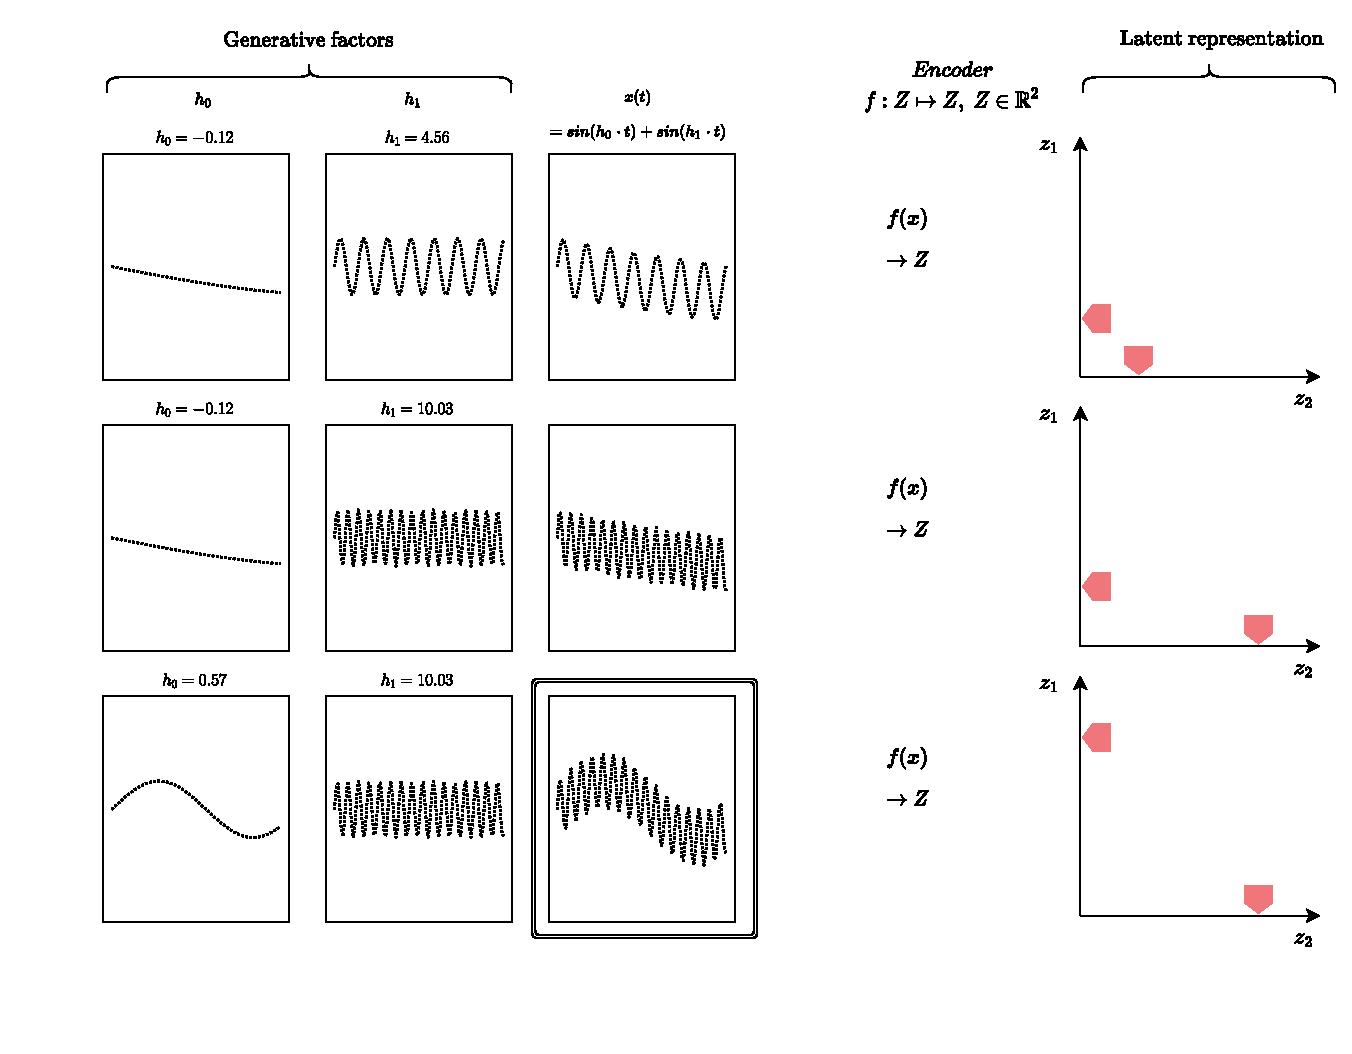
\includegraphics[width=.6\linewidth]{../figures/intution_3x3_3.pdf}
	\caption{Changing values of generating factors are reflected in the corresponding latent variables.}
\end{figure}
%It would provide a remedy to problems such as uninterpretable representation.
\begin{figure}
	\centering
	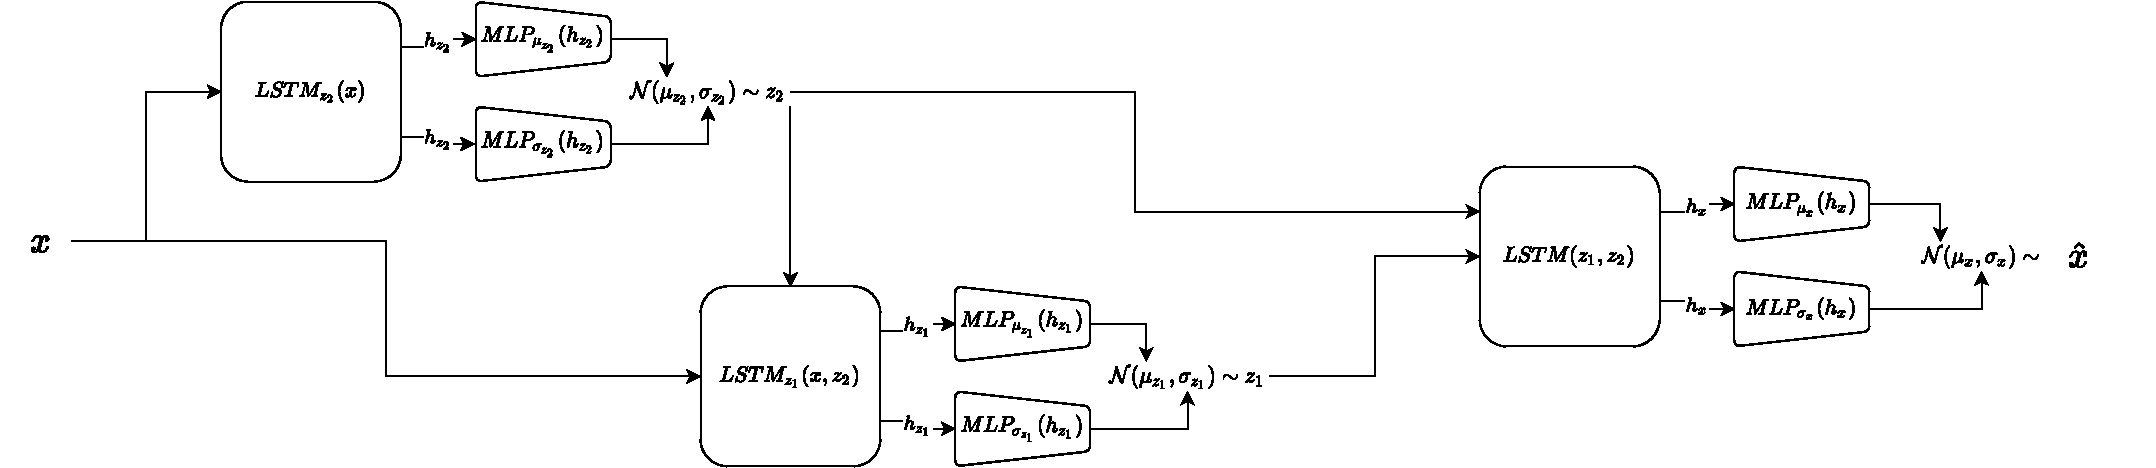
\includegraphics[width=1\linewidth]{../figures/fhvae_complete.pdf}
	\caption{Architecture of the proposed FHVAE.}
\end{figure}
%Since \citet{locatello2019challenging} proved that learning such representations without any supervision or inductive biases is impossible, many works have focused on 

%\lipsum[2-3] (Figure \ref{fig:figure_01}).

%\begin{figure}[h]
%    \includegraphics[width=\textwidth]{figures/figure1.png}
%    \caption{kjsdflkajsdkfjsd}
%    \label{fig:figure_01}
%\end{figure}

\section*{Viewing the FHVAE though a Formal Lense}
%\lipsum[4-6]\cite{Papamakarios2016, Ardizzone2019}
Works on disentanglement often lack a proper formal framework \cite{higgins2018towards}. While claiming to achieve disentanglement, \citet{hsu2017unsupervised} do not provide any formal foundation for their claim. With no formal tools at hand, we cannot formally discuss whether disentanglement was achieved. Thus, we use the following sections to respectively give a theoretical background that defines disentanglement in group theoretic terms, and describe the problem, the FHVAE was designed to solve, in these terms.

\subsection*{The Tools of Group Theory}
A group is described by a tuple of an operation $\circ$ and a non-empty set $G$. The set has to be closed under the operation, it must contain an identity element, the operation must be associative, and for every element in $G$, there must be an inverse element \cite{benkart1987abstract}.
%TODO direct product
Groups can be composed via a direct product. The result of a direct product of groups is itself a group.\\
 A group that is of particular interest for the field of disentangled representation learning is the symmetry group \cite{benkart1987abstract}.
A symmetry group consists of a set of transformations that leave a given object $X$ invariant and the operation is the composition of such transformations. A prominent example of a symmetry group is $SE_3$. This symmetry group can be visualized as a set set of vertices $X$ that form an equilateral triangle. Permutations of this set would result in rotations or flips of the triangle. These permutations would be the symmetry transformations of our symmetry group. The operation would be composing multiple permutations.\\
Another important concept is the group actoin. It is the result of applying a symmetry transformation to an object. In our triangle example, a group action would be the permuted set of vertices.\\




\subsection*{Symmetries in Sequential Data}




\section*{FHVAE - Constructing an Equivariant Map}


\section*{Results}


\section*{Discussion}
Lack of formal context.
Lack of evidence for disentaglement.
Further exploit the available data using cross reconstruction.

\section*{Conclusion}



\newpage
\bibliographystyle{unsrtnat}
\bibliography{refs}

\end{document}
